% This file was created by matplotlib2tikz v0.6.18.
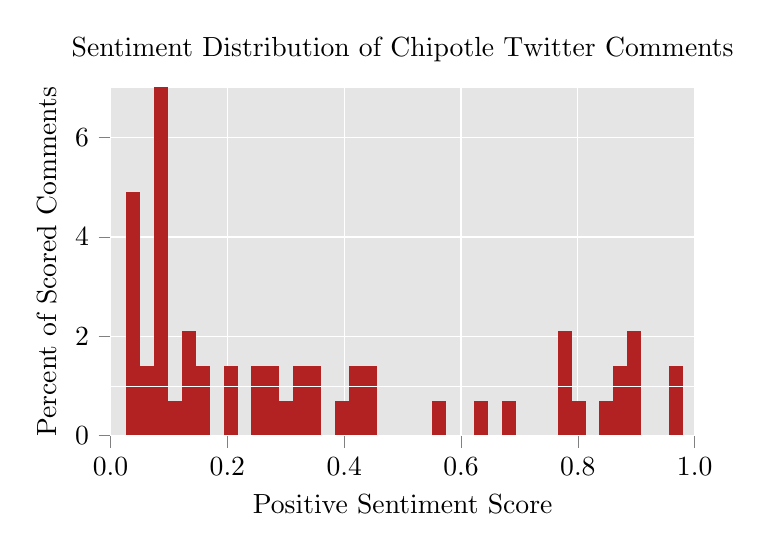
\begin{tikzpicture}

\definecolor{color0}{rgb}{0.698039215686274,0.133333333333333,0.133333333333333}

\begin{axis}[
axis background/.style={fill=white!89.80392156862746!black},
axis line style={white},
height=6cm,
tick align=outside,
tick pos=left,
title={Sentiment Distribution of Chipotle Twitter Comments},
width=9cm,
x grid style={white},
xlabel={Positive Sentiment Score},
xmajorgrids,
xmin=0, xmax=1,
xtick={0,0.2,0.4,0.6,0.8,1},
xticklabels={0.0,0.2,0.4,0.6,0.8,1.0},
y grid style={white},
ylabel={Percent of Scored Comments},
ymajorgrids,
ymin=0, ymax=7
]
\draw[fill=color0,draw opacity=0] (axis cs:0.0266921669244766,0) rectangle (axis cs:0.0505239889025688,4.89541533055737);
\draw[fill=color0,draw opacity=0] (axis cs:0.0505239889025688,0) rectangle (axis cs:0.074355810880661,1.39869009444496);
\draw[fill=color0,draw opacity=0] (axis cs:0.074355810880661,0) rectangle (axis cs:0.0981876254081726,9.79083372203874);
\draw[fill=color0,draw opacity=0] (axis cs:0.0981876254081726,0) rectangle (axis cs:0.122019447386265,0.699345047222482);
\draw[fill=color0,draw opacity=0] (axis cs:0.122019454836845,0) rectangle (axis cs:0.145851284265518,2.09803514166745);
\draw[fill=color0,draw opacity=0] (axis cs:0.145851269364357,0) rectangle (axis cs:0.169683083891869,1.39869053171982);
\draw[fill=color0,draw opacity=0] (axis cs:0.169683068990707,0) rectangle (axis cs:0.19351489841938,0);
\draw[fill=color0,draw opacity=0] (axis cs:0.193514913320541,0) rectangle (axis cs:0.217346727848053,1.39869053171982);
\draw[fill=color0,draw opacity=0] (axis cs:0.217346727848053,0) rectangle (axis cs:0.241178542375565,0);
\draw[fill=color0,draw opacity=0] (axis cs:0.241178527474403,0) rectangle (axis cs:0.265010356903076,1.39869053171982);
\draw[fill=color0,draw opacity=0] (axis cs:0.265010356903076,0) rectangle (axis cs:0.28884220123291,1.39868878262203);
\draw[fill=color0,draw opacity=0] (axis cs:0.28884220123291,0) rectangle (axis cs:0.312674015760422,0.69934526585991);
\draw[fill=color0,draw opacity=0] (axis cs:0.312673985958099,0) rectangle (axis cs:0.336505800485611,1.39869053171982);
\draw[fill=color0,draw opacity=0] (axis cs:0.336505830287933,0) rectangle (axis cs:0.360337644815445,1.39869053171982);
\draw[fill=color0,draw opacity=0] (axis cs:0.360337615013123,0) rectangle (axis cs:0.384169429540634,0);
\draw[fill=color0,draw opacity=0] (axis cs:0.384169459342957,0) rectangle (axis cs:0.408001303672791,0.699344391311017);
\draw[fill=color0,draw opacity=0] (axis cs:0.408001303672791,0) rectangle (axis cs:0.431833118200302,1.39869053171982);
\draw[fill=color0,draw opacity=0] (axis cs:0.43183308839798,0) rectangle (axis cs:0.455664902925491,1.39869053171982);
\draw[fill=color0,draw opacity=0] (axis cs:0.455664932727814,0) rectangle (axis cs:0.479496747255325,0);
\draw[fill=color0,draw opacity=0] (axis cs:0.479496717453003,0) rectangle (axis cs:0.503328561782837,0);
\draw[fill=color0,draw opacity=0] (axis cs:0.503328561782837,0) rectangle (axis cs:0.527160406112671,0);
\draw[fill=color0,draw opacity=0] (axis cs:0.527160406112671,0) rectangle (axis cs:0.55099219083786,0);
\draw[fill=color0,draw opacity=0] (axis cs:0.55099219083786,0) rectangle (axis cs:0.574824035167694,0.699344391311017);
\draw[fill=color0,draw opacity=0] (axis cs:0.574823975563049,0) rectangle (axis cs:0.598655760288239,0);
\draw[fill=color0,draw opacity=0] (axis cs:0.598655819892883,0) rectangle (axis cs:0.622487664222717,0);
\draw[fill=color0,draw opacity=0] (axis cs:0.622487664222717,0) rectangle (axis cs:0.646319508552551,0.699344391311017);
\draw[fill=color0,draw opacity=0] (axis cs:0.646319508552551,0) rectangle (axis cs:0.67015129327774,0);
\draw[fill=color0,draw opacity=0] (axis cs:0.67015129327774,0) rectangle (axis cs:0.693983137607574,0.699344391311017);
\draw[fill=color0,draw opacity=0] (axis cs:0.69398307800293,0) rectangle (axis cs:0.717814862728119,0);
\draw[fill=color0,draw opacity=0] (axis cs:0.717814922332764,0) rectangle (axis cs:0.741646766662598,0);
\draw[fill=color0,draw opacity=0] (axis cs:0.741646766662598,0) rectangle (axis cs:0.765478610992432,0);
\draw[fill=color0,draw opacity=0] (axis cs:0.765478610992432,0) rectangle (axis cs:0.789310395717621,2.09803842123297);
\draw[fill=color0,draw opacity=0] (axis cs:0.789310395717621,0) rectangle (axis cs:0.813142240047455,0.699344391311017);
\draw[fill=color0,draw opacity=0] (axis cs:0.81314218044281,0) rectangle (axis cs:0.836973965167999,0);
\draw[fill=color0,draw opacity=0] (axis cs:0.836974024772644,0) rectangle (axis cs:0.860805869102478,0.699344391311017);
\draw[fill=color0,draw opacity=0] (axis cs:0.860805869102478,0) rectangle (axis cs:0.884637713432312,1.39868878262203);
\draw[fill=color0,draw opacity=0] (axis cs:0.884637713432312,0) rectangle (axis cs:0.908469498157501,2.09803842123297);
\draw[fill=color0,draw opacity=0] (axis cs:0.908469498157501,0) rectangle (axis cs:0.932301342487335,0);
\draw[fill=color0,draw opacity=0] (axis cs:0.93230128288269,0) rectangle (axis cs:0.95613306760788,0);
\draw[fill=color0,draw opacity=0] (axis cs:0.956133127212524,0) rectangle (axis cs:0.979964971542358,1.39868878262203);
\path [draw=white, fill opacity=0] (axis cs:0,0)
--(axis cs:0,7);

\path [draw=white, fill opacity=0] (axis cs:1,0)
--(axis cs:1,7);

\path [draw=white, fill opacity=0] (axis cs:0,0)
--(axis cs:1,0);

\path [draw=white, fill opacity=0] (axis cs:0,1)
--(axis cs:1,1);

\end{axis}
\label{Chipotlet}
\end{tikzpicture}